\Large
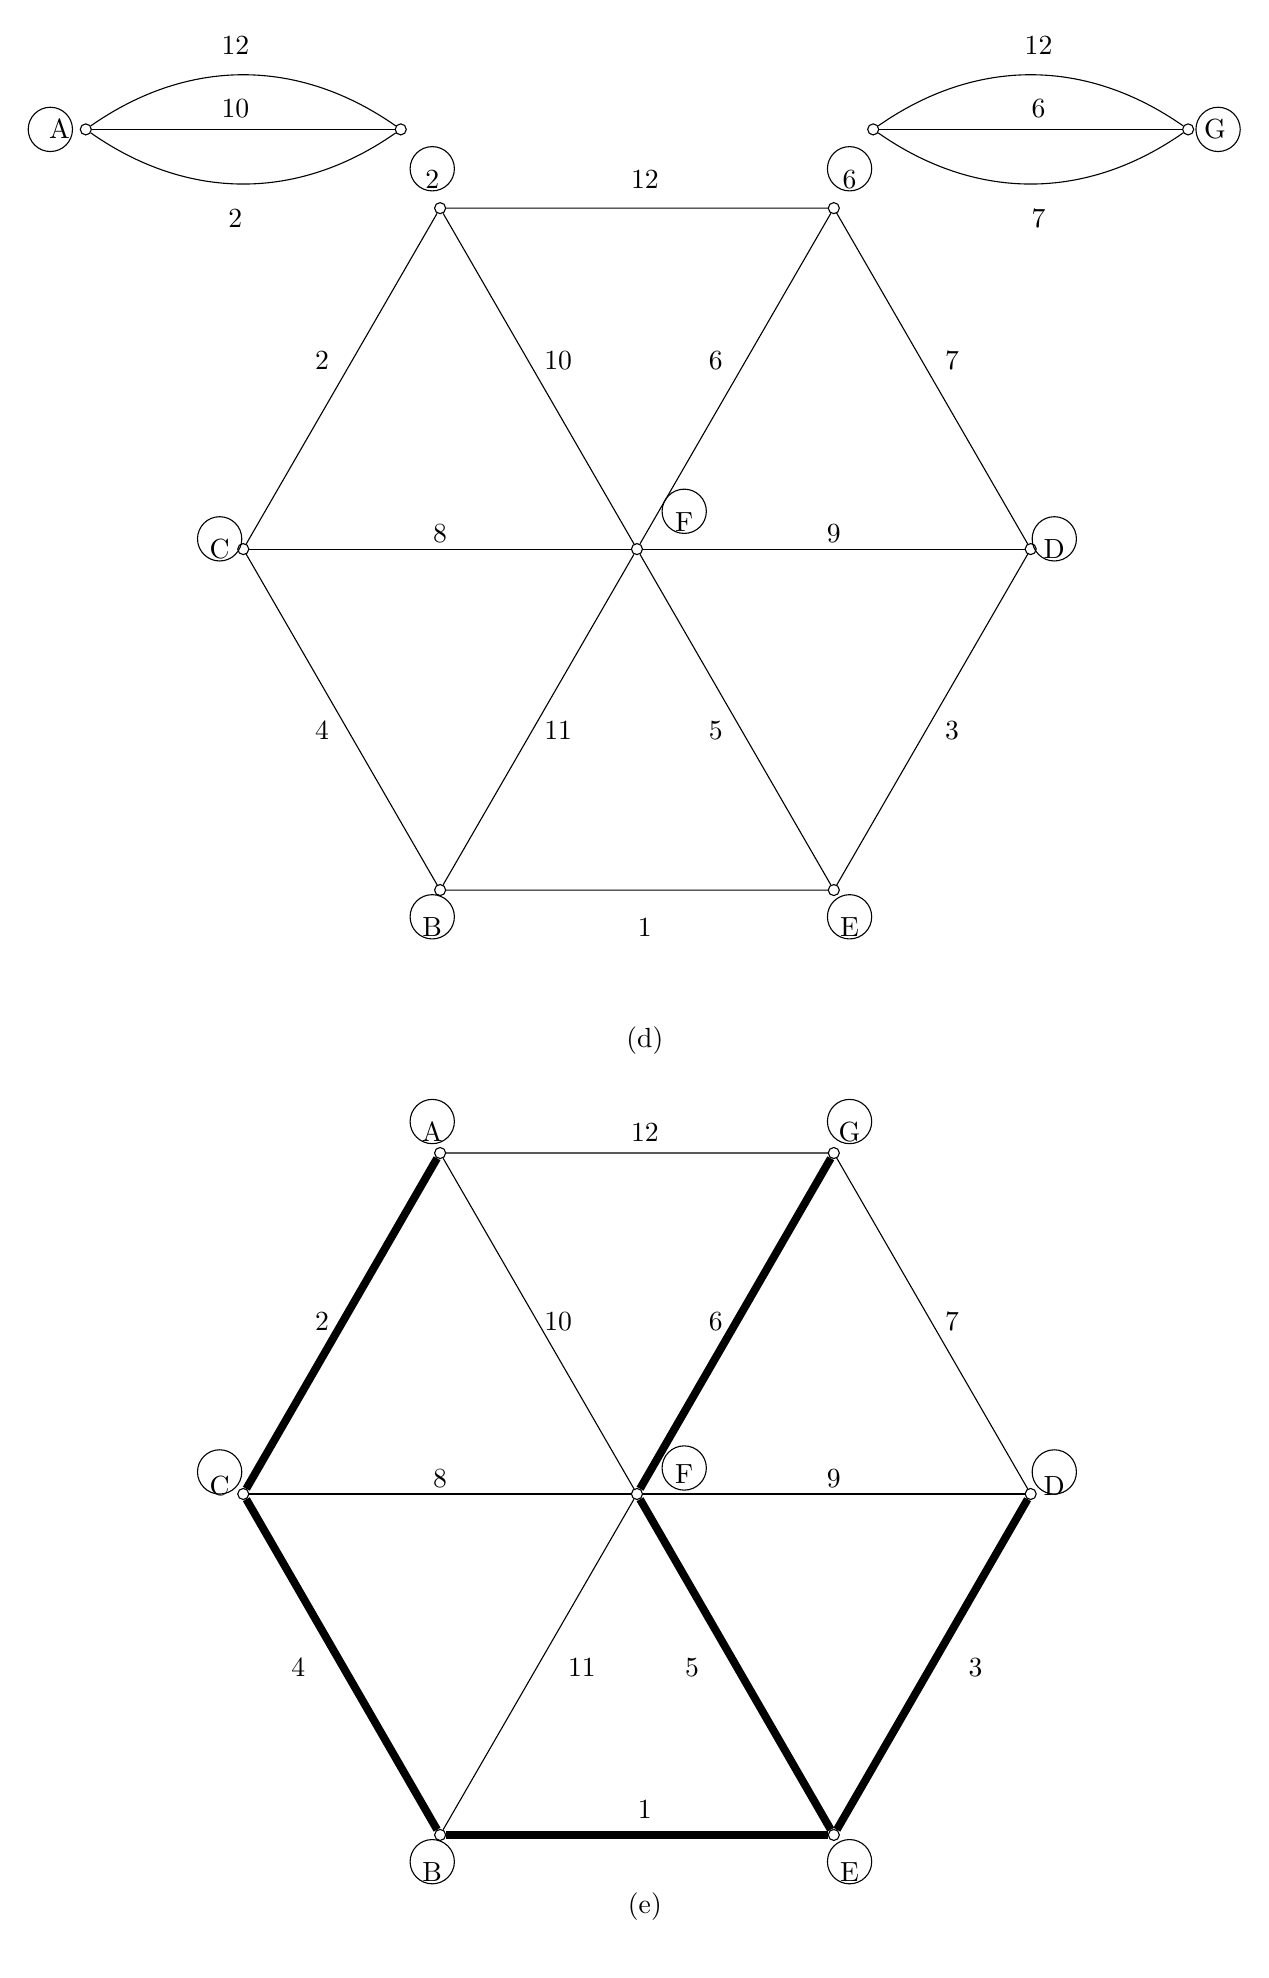
\begin{tikzpicture}
%%%%%%%%%%%%%%%%%%%%%%%%% LEFT TOP GRAPH %%%%%%%%%%%%%%%%%%%%%	
	\draw (-14,+12) 
		node (A1) [draw,circle,fill=white,minimum size=4pt,inner sep=0pt,label=left:A]{}  
		-- ++ (0:4.0cm) 
			node (A2) [draw,circle,fill=white,minimum size=4pt,inner sep=0pt] {};
			\draw (A1) to [out=-35,in=215] (A2);
			\draw (A1) to [out=+35,in=-215] (A2);
			\draw (-14.45,+12) 
				node (LA1) [draw,circle,minimum size=16pt]{};
			\draw (-12.1,+12.7) 
				node (L1)[label=above:12]{};
			\draw (-12.1,+11.9) 
				node (L2) [label=above:10]{};
			\draw (-12.1,+10.5) 
				node (L3) [label=above:2]{};
%%%%%%%%%%%%%%%%%%%%%%%%% RIGHT TOP GRAPH %%%%%%%%%%%%%%%%%%%%%%%
	\draw (-4,+12) 
		node (G1) [draw,circle,fill=white,minimum size=4pt,inner sep=0pt,label=left:] {}  
		-- ++ (0:4.0cm) 
			node (G2) [draw,circle,fill=white,minimum size=4pt,inner sep=0pt, label=right:G] {};
			\draw (G1) to [out=-35,in=215] (G2);
			\draw (G1) to [out=+35,in=-215] (G2);
			\draw (0.38,+12) 
				node (GG1) [draw,circle,minimum size=16pt]{};
			\draw (-1.9,+12.7) 
				node (L4) [label=above:12]{} ;
			\draw (-1.9,+11.9) 
				node (L5) [label=above:6]{} ;
			\draw (-1.9,+10.5) 
				node (L6) [label=above:7]{} ;
%%%%%%%%%%%%%%%%%%%%%%%%% MIDDLE GRAPH %%%%%%%%%%%%%%%%%%%%%%%%%%%%    

     \draw (-9.5,11) node (H1) [draw,circle,fill=white,minimum size=4pt,inner sep=0pt] {}
        -- ++(0:5.0cm) node (H2) [draw,circle,fill=white,minimum size=4pt,inner sep=0pt] {}
        -- ++(300:5.0cm) node (H3) [draw,circle,fill=white,minimum size=4pt,inner sep=0pt] {}
        -- ++(240:5.0cm) node (H4) [draw,circle,fill=white,minimum size=4pt,inner sep=0pt] {}
        -- ++(180:5.0cm) node (H5) [draw,circle,fill=white,minimum size=4pt,inner sep=0pt] {}
        -- ++(120:5.0cm) node (H6) [draw,circle,fill=white,minimum size=4pt,inner sep=0pt] {}
        -- (H1) % shape is closed, we now connect it to an outer vertex:
        -- ++(300:5.0cm) node (H7) [draw,circle,fill=white,minimum size=4pt,inner sep=0pt] {};
		\draw (H2) -- (H7);
		\draw (H3) -- (H7);
		\draw (H4) -- (H7);
		\draw (H5) -- (H7);
		\draw (H6) -- (H7);
		\draw (-9.6,+11.0) node (HL01) [label=above:2]{};
		\draw (-9.6,+11.5) node (HG1) [draw,circle,minimum size=16pt]{};
		\draw (-4.3,+11.0) node (HL02) [label=above:6]{};  
		\draw (-4.3,+11.5) node (HG2) [draw,circle,minimum size=16pt]{};
		\draw (-12.3,+6.3) node (HL03) [label=above:C]{};  
		\draw (-12.3,+6.8) node (HG3) [draw,circle,minimum size=16pt]{};
		\draw (-1.7,+6.3) node (HL04) [label=above:D]{};  
		\draw (-1.7,+6.8) node (HG4) [draw,circle,minimum size=16pt]{};
		\draw (-6.4,+6.65) node (HL05) [label=above:F]{};  
		\draw (-6.4,+7.15) node (HG5) [draw,circle,minimum size=16pt]{};
		\draw (-9.6,+1.5) node (HL06) [label=above:B]{};
		\draw (-9.6,+2.0) node (HG6) [draw,circle,minimum size=16pt]{};
		\draw (-4.3,+1.5) node (HL07) [label=above:E]{};  
		\draw (-4.3,+2.0) node (HG7) [draw,circle,minimum size=16pt]{};
		\draw (-6.9,+11.0) node (HL1) [label=above:12]{};
		\draw (-11.0,+8.7) node (HL2) [label=above:2]{};
		\draw (-8.0,+8.7) node (HL3) [label=above:10]{}; 
		\draw (-6.0,+8.7) node (HL4) [label=above:6]{};
		\draw (-3.0,+8.7) node (HL5) [label=above:7]{};
		\draw (-9.5,+6.5) node (HL6) [label=above:8]{};
		\draw (-4.5,+6.5) node (HL7) [label=above:9]{};
		\draw (-11.0,+4.0) node (HL8) [label=above:4]{};
		\draw (-8.0,+4.0) node (HL9) [label=above:11]{}; 
		\draw (-6.0,+4.0) node (HL10) [label=above:5]{};
		\draw (-3.0,+4.0) node (HL11) [label=above:3]{};
		\draw (-6.9,+1.5) node (HL12) [label=above:1]{}; 
		\draw (-6.9,0.0) node (HL99) [label=above:(d)]{}; 
%%%%%%%%%%%%%%%%%%%%%%%%% BOTTOM GRAPH %%%%%%%%%%%%%%%%%%%%%%%%%%%%    
		
     \draw (-9.5,-1.0) node (H21) [draw,circle,fill=white,minimum size=4pt,inner sep=0pt] {}
        -- ++(0:5.0cm) node (H22) [draw,circle,fill=white,minimum size=4pt,inner sep=0pt] {}
        -- ++(300:5.0cm) node (H23) [draw,circle,fill=white,minimum size=4pt,inner sep=0pt] {}
        -- ++(240:5.0cm) node (H24) [draw,circle,fill=white,minimum size=4pt,inner sep=0pt] {}
        -- ++(180:5.0cm) node (H25) [draw,circle,fill=white,minimum size=4pt,inner sep=0pt] {}
        -- ++(120:5.0cm) node (H26) [draw,circle,fill=white,minimum size=4pt,inner sep=0pt] {}
        -- (H21) % shape is closed, we now connect it to an outer vertex:
        -- ++(300:5.0cm) node (H27) [draw,circle,fill=white,minimum size=4pt,inner sep=0pt] {};

		\draw (H22)[line width=1mm] -- (H27);
		\draw (H21)[line width=1mm] -- (H26);
		\draw (H23) -- (H27);
		\draw (H24)[line width=1mm] -- (H27);
		\draw (H25) -- (H27);
		\draw (H26) -- (H27);
		\draw (H25)[line width=1mm] -- (H26);
		\draw (H24)[line width=1mm] -- (H25);
		\draw (H23)[line width=1mm] -- (H24);
		\draw (-9.6,-10.5) node (HL201) [label=above:B]{};
		\draw (-9.6,-10.0) node (HG21) [draw,circle,minimum size=16pt]{};
		\draw (-4.3,-10.5) node (HL202) [label=above:E]{};  
		\draw (-4.3,-10.0) node (HG22) [draw,circle,minimum size=16pt]{};
		\draw (-12.3,-5.6) node (HL203) [label=above:C]{};  
		\draw (-12.3,-5.05) node (HG23) [draw,circle,minimum size=16pt]{};
		\draw (-1.7,-5.6) node (HL204) [label=above:D]{};  
		\draw (-1.7,-5.05) node (HG24) [draw,circle,minimum size=16pt]{};
		\draw (-6.4,-5.45) node (HL05) [label=above:F]{};  
		\draw (-6.4,-5.0) node (HG5) [draw,circle,minimum size=16pt]{};
		\draw (-9.6,-1.1) node (HL206) [label=above:A]{};
		\draw (-9.6,-0.6) node (HG26) [draw,circle,minimum size=16pt]{};
		\draw (-4.3,-1.1) node (HL207) [label=above:G]{};  
		\draw (-4.3,-0.6) node (HG27) [draw,circle,minimum size=16pt]{};
		\draw (-6.9,-1.1) node (HL21) [label=above:12]{};
		\draw (-11.0,-3.5) node (HL22) [label=above:2]{};
		\draw (-8.0,-3.5) node (HL23) [label=above:10]{};
		\draw (-6.0,-3.5) node (HL24) [label=above:6]{};
		\draw (-3.0,-3.5) node (HL25) [label=above:7]{};
		\draw (-9.5,-5.5) node (HL26) [label=above:8]{};
		\draw (-4.5,-5.5) node (HL27) [label=above:9]{};
		\draw (-11.3,-7.9) node (HL28) [label=above:4]{};
		\draw (-7.7,-7.9) node (HL29) [label=above:11]{};
		\draw (-6.3,-7.9) node (HL210) [label=above:5]{};
		\draw (-2.7,-7.9) node (HL211) [label=above:3]{};
		\draw (-6.9,-9.7) node (HL212) [label=above:1]{};
		\draw (-6.9,-11.0) node (HL213) [label=above:(e)]{};
\end{tikzpicture}


